\documentclass[conference]{IEEEtran}
\IEEEoverridecommandlockouts
\renewcommand\IEEEkeywordsname{Keywords}
% The preceding line is only needed to identify funding in the first footnote. If that is unneeded, please comment it out.
%for tables

\usepackage{booktabs}
\usepackage{multirow}
%end for tables
\usepackage{cite}
\usepackage{balance}

\usepackage{amsmath,amssymb,amsfonts} %Mathematical Symbol,Equation
\usepackage{hyperref}
\hypersetup{
    colorlinks=true,
    linkcolor=blue,
    filecolor=magenta,
    urlcolor=cyan,
    citecolor=green,
    pdftitle={Handling Extensive Missingness in Newspaper-Reported Suicide Data},
    }
\usepackage{graphicx} %Adding picture \& figure
\graphicspath{{figures/}}
\usepackage{float} %Figure Alignment
\usepackage{pgfplots} %Native vector bar chart (Results)
\usetikzlibrary{patterns,positioning} %Hatched overlay and relative placement on the missingness heatmap
\pgfplotsset{compat=1.17}
\usepackage{algorithm}      %Algorithm float (Methodology pseudocode)
\usepackage{algpseudocode}  %Pseudocode commands
\usepackage{textcomp} %Text formatting
\usepackage{eso-pic}
\usepackage{xcolor}
\definecolor{figblue}{HTML}{004C99} % shared accent for both pgfplots charts
\usepackage{comment}
\usepackage{csquotes}
\usepackage{tabularx}
\def\BibTeX{{\rm B\kern-.05em{\sc i\kern-.025em b}\kern-.08em
    T\kern-.1667em\lower.7ex\hbox{E}\kern-.125emX}}

\makeatletter
%%%%%%%%%%%%%%%%%%%%%%%%%%%%%% User specified LaTeX commands.

\newcommand{\snippet}[1]{``\texttt{#1}''}



\usepackage{eso-pic}
\newcommand\AtPageUpperMyright[1]{\AtPageUpperLeft{%
 \put(\LenToUnit{0.5\paperwidth},\LenToUnit{-1cm}){%
     \parbox{0.5\textwidth}{\raggedleft\fontsize{9}{11}\selectfont #1}}%
 }}%
\newcommand{\conf}[1]{%
\AddToShipoutPictureBG*{%
\AtPageUpperMyright{#1}
}
}
%\hyphenation{op-tical net-works semi-conduc-tor}
\usepackage{fancyhdr}

\setlength {\marginparwidth }{2cm}

\makeatletter
\def\footnoterule{\kern-3\p@
  \hrule \@width 2in \kern 2.6\p@} % the \hrule is .4pt high
\makeatother

\begin{document}

% Creating a custom header for the first page
\makeatletter

% Header settings

\title{Addressing Extensive Missingness in Newspaper-Reported Suicide Data Through Imputation and Clustering Techniques}

% TODO (before submission): confirm supervisor email address.
% Author order: student (corresponding) first, supervisor last.

\author{\IEEEauthorblockN{Mohammed Akash, Sajedul Islam, Nusrat Kaniz Khan, and Md. Mamun Hossain}

\IEEEauthorblockA{\textit{Department of Computer Science and Engineering} \\
\textit{Bangladesh University of Business and Technology, Dhaka (BUBT), Bangladesh} \\
21221203019@cse.bubt.edu.bd, 21221203022@cse.bubt.edu.bd,  nusrat002.mist@gmail.com \& mamunhasan.cs@gmail.com }}

\maketitle


% The paper headers and footers
\thispagestyle{fancyplain}
\fancyhf{}
\rhead{\fancyplain{}{11th IEEE Asia-Pacific Conference on Computer Science and Data Engineering (IEEE CSDE2026)\\1-3 November 2026, Cox’s Bazar, Bangladesh}}
% TODO (before submission): insert assigned IEEE copyright/DOI string when registration finalises it.
\lfoot{\fancyplain{}{979-8-3195-4477-3/26/\$31.00 ©2026 IEEE}}
\renewcommand{\headrulewidth}{0pt}

%%%%%%%%%%%%%%%%%%%%%%%%%%%%%%%%%%%%%%%%%%%%%%%%%%%%%%%%%%%%%%%%%%%%%%%%%%%%%%%%
\begin{abstract}
In countries without a central suicide registry, newspaper reports are often the only public source of case-level data, yet they are severely incomplete, with missingness reaching 90\% on the sparsest fields. We assemble 1{,}617 newspaper-reported suicide cases from Bangladesh (2017--2025), extending a public collection with newly collected cases, and ask whether principled imputation can make such data usable for unsupervised analysis. Our pipeline first consolidates the raw free-text labels into a compact vocabulary (918 values reduced to 156 categories), then benchmarks three imputers (MissForest, MICE, and $k$-nearest neighbours) against two clustering algorithms (K-Means and Agglomerative) under a six-component, balance-aware cluster-validity score. Each imputed cell is compared against no-imputation baselines that simply drop the incomplete columns and rows, giving ten pipelines. Rather than fix one weighting of the six metrics, we test robustness directly. Across 100{,}000 weight vectors sampled uniformly over the metric simplex, the four strong imputed pipelines occupy the top four ranks in over 99.9\% of weightings, while the two poorly-combined imputed pipelines and all four baselines are essentially never among the best. Imputation therefore helps regardless of the weighting. The gain still depends on the pairing of imputer and clustering algorithm, and two imputed pipelines fall below the best baseline. We report no single best pipeline, yet the strong pipelines converge on the same clean, cohort-aligned two-cluster structure. Careful imputation is a feasible foundation for suicide surveillance in low-resource, news-derived public-health data.
\end{abstract}


%\vspace{2mm}
\begin{IEEEkeywords}
\textcolor{black}{\textit{imputation; clustering; missing data; suicide; MissForest; public health; Bangladesh}}
\end{IEEEkeywords}


\section{Introduction}
\label{sec:Introduction}

Suicide is a leading cause of death among young people and an explicit concern of the United Nations Sustainable Development Goals. Target 3.4 of Goal 3 (SDG-3) calls for a one-third reduction in premature mortality from non-communicable diseases and mental-health conditions by 2030, and the suicide mortality rate is tracked as indicator~3.4.2~\cite{un2015sdg,who2024sdg34}. Effective prevention depends on case-level surveillance data that many low- and middle-income countries (LMICs) do not systematically collect. National suicide registries are absent or fragmentary, and where suicide is criminalised the official records are further suppressed~\cite{arafat2025surveillance}. In Bangladesh, as in many LMICs, newspaper reports are among the only public sources of case-level information on suicide, and they have been used to study its demography and risk factors~\cite{himel2024studentnews}.

News-derived data, however, are ill-suited to standard machine-learning workflows. Reporting is incidental rather than systematic, so many key fields (occupation, location, financial circumstances, prior mental-health history) are missing for roughly half to over 90\% of cases in the raw reports, and the missingness is structured rather than random. Listwise deletion is not viable. In our corpus only $3.5\%$ of records are complete across all retained fields, so dropping incomplete rows would discard the overwhelming majority of the data, while restricting to the few well-populated columns throws away most of the feature space. The practical question for surveillance in this regime is therefore not which model to fit, but whether the data can be made usable at all.

We address this with a transparent pipeline on a dataset of 1{,}617 newspaper-reported suicide cases from Bangladesh (2017 to 2025). The pipeline first consolidates the raw free-text categorical labels into a compact canonical vocabulary. It then benchmarks three imputation methods against two clustering algorithms under a six-component composite score that rewards well-balanced clusters. We also compare each imputed pipeline against a no-imputation baseline that simply drops the incomplete columns and rows. The study asks whether such a pipeline can surface stable and interpretable structure in severely incomplete newspaper data, and how this compares with dropping the incomplete records instead.

This study pursues three objectives.
\begin{itemize}
\item To construct a comprehensive dataset of newspaper-reported suicide cases in Bangladesh by extending an existing public dataset with newly collected records.
\item To systematically evaluate the effectiveness of different imputation and clustering method combinations against no-imputation baselines using a balance-aware cluster-validity metric.
\item To examine the robustness of imputation-based clustering performance across diverse metric weightings and identify the most effective imputation--clustering combinations.
\end{itemize}

\section{Related Works}
\label{sec:related-works}

Newspaper reports are widely used to monitor suicide in low- and middle-income countries (LMICs) where official data are limited. Arafat~\cite{arafat2025surveillance} notes that many LMICs lack a central suicide registry, and that criminalisation further suppresses official records, leaving news reports as a primary public source. That work argues for surveillance reform rather than a computational pipeline for the resulting data. Himel et al.~\cite{himel2024studentnews} analyse post-pandemic student suicides from Bangladeshi online news, the same medium and country as ours. Their study is descriptive and manual. It shows that newspapers are a viable substrate but leaves their severe, structured missingness untreated. That gap is what we address.

The three estimators we benchmark, MissForest, MICE, and $k$-nearest-neighbour imputation, are the field's de facto baselines, and we detail and cite them in Section~\ref{sec:Methodology}. Broad imputation benchmarks tend to favour iterative, model-based methods on mixed-type data~\cite{jager2021benchmark}, and imputation quality has measurable downstream effects on classifiers~\cite{shadbahr2023imputationquality}. Both, however, use complete data with artificially induced missingness and withheld ground truth. Prakash et al.~\cite{prakash2025mentalhealthimpute} benchmark imputation on large-scale mental-health surveys, the closest domain to ours, but again on artificially removed values. Closest in spirit, Aracri et al.~\cite{aracri2025imputation} compare KNN, MICE, and MissForest on dementia data and, like us, judge them by a downstream task rather than by per-cell reconstruction.

Clustering is widely used to find subgroups in suicide and mental-health data. Sanz-Gomez et al.~\cite{sanzgomez2025impulsivity} profiled suicide deaths with k-means, Namgung et al.~\cite{namgung2024subgroups} separated psychiatric outpatients into risk subgroups, and Wong et al.~\cite{wong2022studentclusters} classified student suicides into typologies. All operate on largely complete clinical or registry records, not the severely incomplete news data treated here. With no ground-truth labels, internal cluster-validity indices stand in. The silhouette~\cite{rousseeuw1987silhouette} is the most common, and Chicco et al.~\cite{chicco2025silhouette} show that no single index suffices and that silhouette and Davies--Bouldin are often the most informative, which motivates our multi-index composite.

Each thread covers only part of this space. News-based suicide studies do neither imputation nor a clustering benchmark. Clustering studies use largely complete records. Imputation benchmarks use complete data with artificial missingness. To our knowledge this paper is among the first to combine news-derived suicide data with a multi-method imputation benchmark, multi-algorithm clustering, released code, and an explicit source-cohort confound analysis.


\section{Methodology}
\label{sec:Methodology}


This section describes the dataset and how we prepared it. It then details the modelling pipeline that produces and scores the clustering results. A final subsection summarises the whole procedure as an algorithm.

\subsection{Data Description and Preprocessing}
The dataset contains 1{,}617 newspaper-reported suicide cases from Bangladesh. We started from a public 2020 collection of 760 cases~\cite{alom2020bangladesh} and added 857 cases that we collected by hand for 2017 to 2019 and 2021 to 2025. To find these cases we searched the web for suicide-related terms such as \snippet{suicide in Bangladesh} and \snippet{Bangladesh suicide 2021}, filtered the results by year and often by news, and read each report before recording it. The reports came from Bangladeshi online newspapers and news portals, such as Prothom Alo, The Daily Star, Jugantor, and Ittefaq. We kept only cases from inside Bangladesh, and only reports of a confirmed completed suicide.

Several team members shared the work, each taking a set of years and going month by month, so no two people covered the same period and duplicates were unlikely. One author then reviewed every case by its reported name, date, and location to remove any remaining duplicates and fix inconsistent entries. We did not compute a formal inter-rater score, since the years were split rather than coded twice. By reported year the corpus is uneven and dominated by 2020 (762 cases), followed by 2022 (313), 2024 (235), 2021 (152), and 2019 (88). After dropping the sparsest fields we kept 29 analytical features, 13 categorical and 16 numerical. Figure~\ref{fig:missingness} shows the per-column missing rate for each field.

\begin{figure}[H]
\centering
\resizebox{\columnwidth}{!}{%
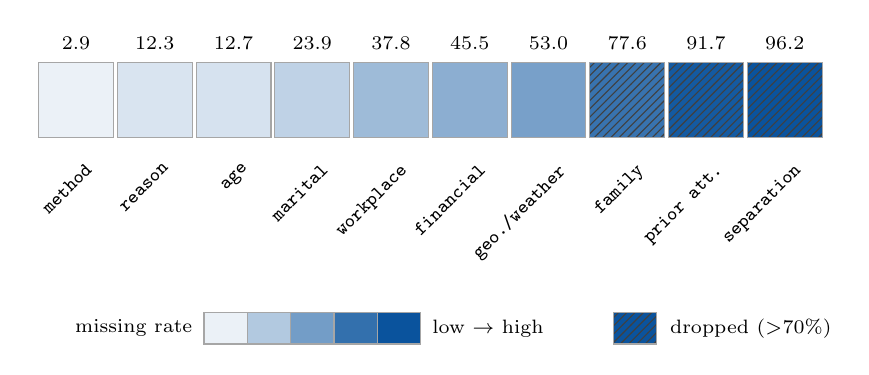
\begin{tikzpicture}[
  tile/.style={draw=black!35,minimum width=0.95cm,minimum height=0.95cm,inner sep=0pt},
  hatch/.style={pattern=north east lines,pattern color=black!75},
  vlbl/.style={font=\scriptsize\ttfamily,rotate=45,anchor=north east},
]
\foreach \i/\lab/\pct/\intensity/\drop in {%
  0/method/2.9/8/0,%
  1/reason/12.3/15/0,%
  2/age/12.7/16/0,%
  3/marital/23.9/25/0,%
  4/workplace/37.8/38/0,%
  5/financial/45.5/45/0,%
  6/{geo./weather}/53.0/53/0,%
  7/family/77.6/78/1,%
  8/{prior att.}/91.7/92/1,%
  9/separation/96.2/96/1%
}{%
  \node[tile,fill=figblue!\intensity!white] (t\i) at (\i*1.0,0) {};
  \ifnum\drop=1
    \node[tile,hatch] at (\i*1.0,0) {};
  \fi
  \node[font=\scriptsize,above=1pt of t\i] {\pct};
  \node[vlbl] at ([xshift=3pt,yshift=-4pt]t\i.south) {\lab};
}
\begin{scope}[shift={(0,-2.9)}]
  \node[font=\scriptsize,anchor=east] at (1.6,0) {missing rate};
  \node[tile,fill=figblue!8!white,minimum width=0.55cm,minimum height=0.4cm] (g1) at (1.9,0) {};
  \node[tile,fill=figblue!30!white,minimum width=0.55cm,minimum height=0.4cm] (g2) at (2.45,0) {};
  \node[tile,fill=figblue!55!white,minimum width=0.55cm,minimum height=0.4cm] (g3) at (3.00,0) {};
  \node[tile,fill=figblue!80!white,minimum width=0.55cm,minimum height=0.4cm] (g4) at (3.55,0) {};
  \node[tile,fill=figblue!96!white,minimum width=0.55cm,minimum height=0.4cm] (g5) at (4.10,0) {};
  \node[font=\scriptsize,anchor=west] at (4.40,0) {low $\rightarrow$ high};
  \node[tile,fill=figblue!96!white,minimum width=0.55cm,minimum height=0.4cm] (gd) at (7.10,0) {};
  \node[tile,hatch,minimum width=0.55cm,minimum height=0.4cm] at (gd) {};
  \node[font=\scriptsize,anchor=west] at (7.42,0) {dropped ($>$70\%)};
\end{scope}
\end{tikzpicture}%
}
\caption{Per-column missing rate in the raw corpus. Shade encodes the rate and hatched tiles mark fields dropped above the $70\%$ threshold.}
\label{fig:missingness}
\end{figure}

Missingness is severe and structured, and it is the dominant modelling obstacle. Per-column missing rates range from under 3\% on the best-reported fields, such as method, reason, and age, to over 90\% on the sparsest. Five fields sat above the 70\% threshold and were dropped, including prior suicide attempt at 91.7\% and duration of separation at 96.2\%. Because these fields are removed rather than filled, imputation never runs on the sparsest data. It only fills the fields that remain below the threshold. The gaps are not random. Sensitive or hard-to-verify fields are almost always absent, and geolocation and weather fields tend to be missing together, which points to a missing-not-at-random (MNAR) mechanism. Listwise deletion is therefore not viable. Only 57 records (3.5\%) are complete across all retained columns. Keeping only the columns below 20\% missingness leaves 853 complete records (52.8\%), and a 40\% threshold leaves only 403 (24.9\%).

The free-text categorical fields were high in cardinality, with 918 unique values across 11 fields, along with typos and verbose descriptions. We consolidated them into 156 canonical categories, an 83\% reduction. We fixed spelling and casing, reduced place names to the home district, and grouped rare categories into broader ones. For example, small groups such as Chakma, Marma, and Santal were merged into a single indigenous religion category alongside the major religions. A large language model (GPT-4) proposed the mappings, and the authors reviewed all 156 and overrode the model in three cases. The model was used only at design time, and the mappings ship as deterministic dictionaries, so the pipeline stays reproducible.

Before imputation, a deterministic recovery stage filled values that external sources make verifiable rather than estimated. Place names were geocoded to latitude and longitude, which cut their missingness from about 53\% to 6.5\%. A Unix timestamp was derived from the reported date and time, dropping from 52.4\% to 5\%. Weather was retrieved from the Meteostat API keyed on location and timestamp, which reduced temperature missingness from 53\% to about 30\%. A few fields such as humidity could not be recovered.

The 29 features were then encoded into two numeric forms. For the distance-based imputers KNN and MICE, the three low-cardinality nominal fields (gender, workplace, religion) were one-hot encoded into one binary column per category. This expands the three fields into eleven columns and gives a 37-column matrix ($29-3+11$). The high-cardinality fields were frequency encoded to avoid the dimensional blow-up of one-hot on many-valued features~\cite{pargent2022highcardinality}. For MissForest, which handles categoricals natively, all 29 features were label encoded, keeping one column per feature.

This recovery stage is shared by every downstream dataset, so the study reduces to a single controlled decision about the columns that remain severely incomplete. The impute arm keeps those columns and fills them statistically. The drop arm discards columns above a missingness threshold, either 20\% or 40\%, and then keeps only complete rows. Table~\ref{tbl:design} lists the five resulting datasets. MICE keeps 1{,}613 rows because four records lacked usable predictors. Any later difference between the arms comes from the imputation choice and not from preprocessing.

\begin{table}[H]
\centering
\footnotesize
\caption{The five datasets entering the benchmark. Each is clustered by both algorithms to give the ten pipelines.}
\label{tbl:design}
\renewcommand{\arraystretch}{1.1}
\begin{tabular*}{\columnwidth}{@{\extracolsep{\fill}}lrrl@{}}
\toprule
\textbf{Dataset} & \textbf{Rows} & \textbf{Cols.} & \textbf{Treatment} \\
\midrule
MissForest   & 1,617 & 29 & imputed (label enc.) \\
MICE         & 1,613 & 37 & imputed (one-hot $+$ freq.) \\
KNN          & 1,617 & 37 & imputed (one-hot $+$ freq.) \\
None (20\%)  &   853 & 22 & drop cols.\ $>$20\%, then rows \\
None (40\%)  &   403 & 30 & drop cols.\ $>$40\%, then rows \\
\bottomrule
\end{tabular*}
\end{table}

\subsection{Architecture}
This subsection details the modelling pipeline, and Fig.~\ref{fig:pipeline} gives the overview.

\begin{figure}[H]
  \centering
  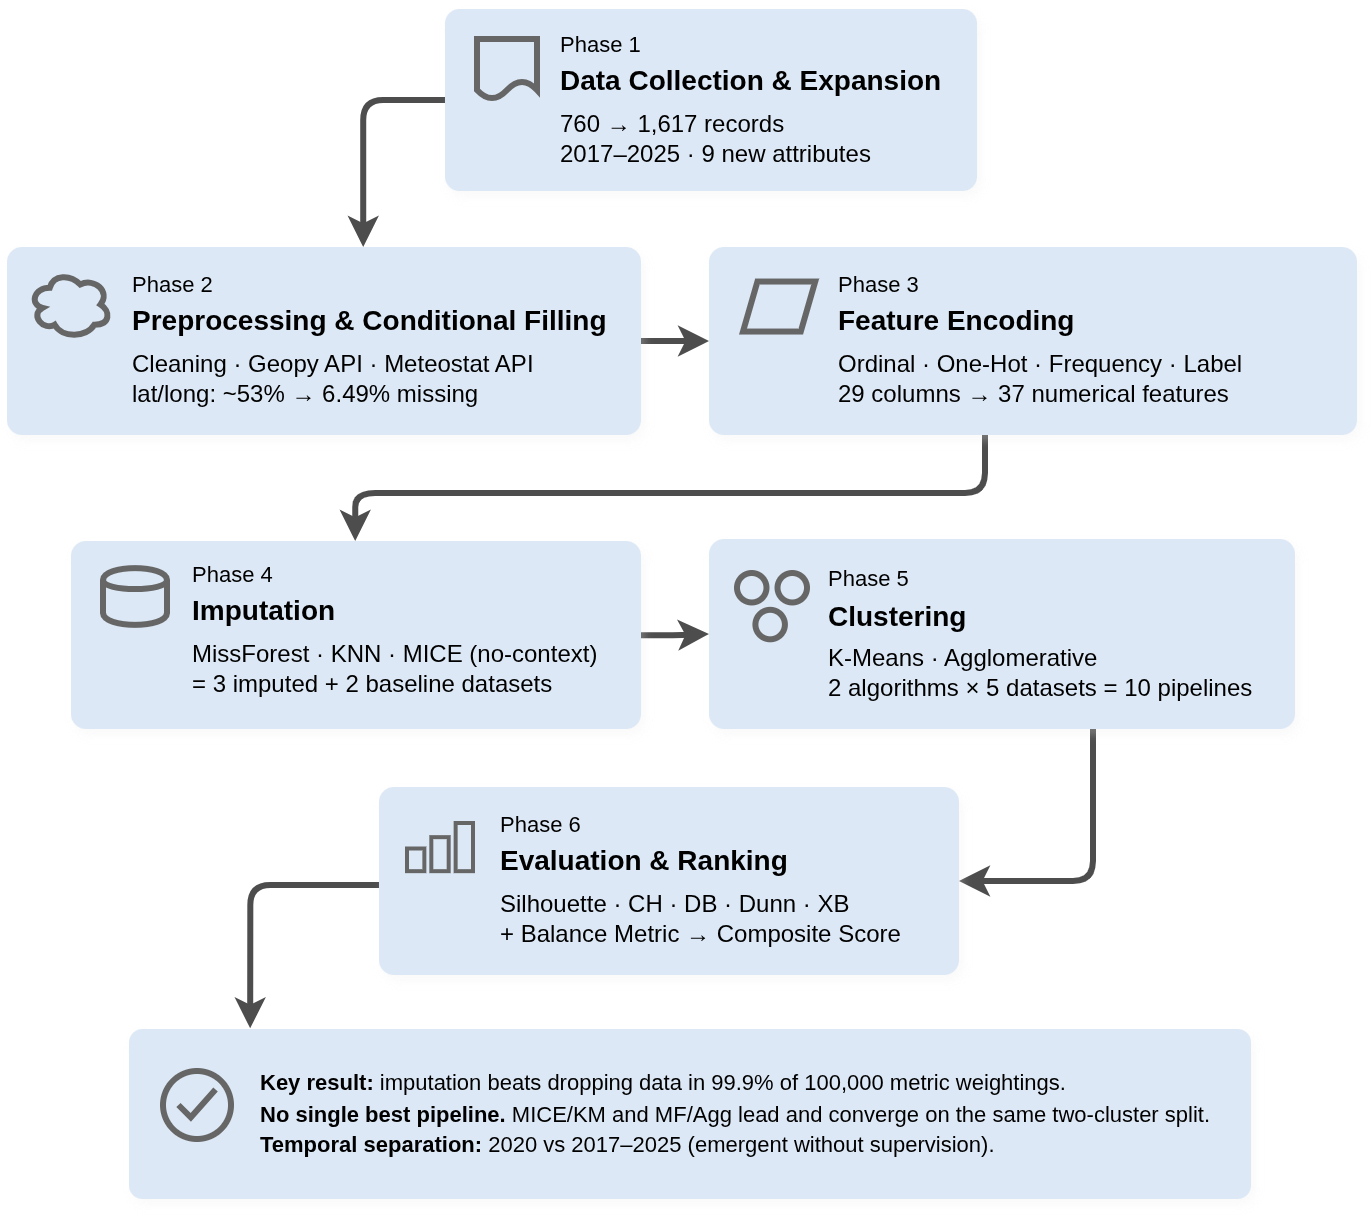
\includegraphics[width=\columnwidth,keepaspectratio]{intro.png}
  \caption{High-level study pipeline, from data collection and preprocessing through encoding, the five datasets, clustering, and composite scoring.}
  \label{fig:pipeline}
\end{figure}

The pipeline takes the cleaned and encoded data, forms the five datasets, clusters each one with K-Means and Agglomerative, and ranks the ten pipelines by the composite score. We describe the imputation, clustering, and scoring steps below.

\subsubsection{Imputation}
We evaluated three imputers from different paradigms, since no single imputer dominates across data types and missingness patterns~\cite{jager2021benchmark}. Each imputer used every available feature as a predictor and produced one imputed dataset. MissForest~\cite{stekhoven2012missforest} ran with 100 trees on the 29 label-encoded columns and iterated to the Stekhoven stopping criterion. KNN imputation~\cite{troyanskaya2001knn} used $k=5$ with Euclidean distance on the 37 one-hot columns. MICE~\cite{vanbuuren2011mice} used a per-variable Bayesian ridge estimator in a single pass over the same columns. All stochastic parts used a fixed seed, and residual missingness stayed below 0.25\%.

\subsubsection{Clustering}
Each dataset was standardised and then reduced with PCA before clustering. We kept 99\% of the variance for K-Means and ten components for Agglomerative. This matters because the matrix mixes one-hot, frequency, and label encodings, and standardisation with PCA places them on comparable scales for Euclidean distance. K-Means~\cite{macqueen1967kmeans} was tuned by grid search over the number of clusters from 2 to 20, the initialisation, the number of initialisations, and the iteration limit. Agglomerative clustering with Ward-style linkage~\cite{ward1963hierarchical} was tuned over linkage and distance metric with the number of clusters from 2 to 10. These two cover the centroid-based and hierarchical families, and using different paradigms guards against mistaking an artefact of one method for real structure.

\subsubsection{Score}
With no ground-truth labels, we ranked pipelines by an internal composite. It combines five standard validity indices (silhouette, Calinski--Harabasz, Dunn, and the inverted Davies--Bouldin and Xie--Beni) with a study-specific balance penalty. The balance term rewards even cluster sizes and penalises over-segmentation, because the geometric indices alone reward near-degenerate partitions such as one huge cluster with a few orphan points. For a partition into $K\geq2$ clusters, where $p_k$ is the share of records in cluster $k$, it is
\begin{equation}\label{eq:balance}
\text{balance} = \left(1 - \sqrt{\tfrac{1}{K}\sum_{k=1}^{K}\Bigl(p_k - \tfrac{1}{K}\Bigr)^{2}}\,\right)\frac{1}{\sqrt{K}},
\end{equation}
The first factor falls as the cluster sizes grow uneven, and the $1/\sqrt{K}$ factor falls as the number of clusters grows. Balance is therefore highest for even, moderately segmented partitions.

The composite works on ranks rather than raw values, since the six metrics live on very different scales. On each metric the ten pipelines are ranked, and the best earns 10 points, the next 9, down to 1 for the worst. With $r_m$ the zero-indexed rank on metric $m$ (so the best pipeline has $r_m=0$) and $n=10$, the score is
\begin{equation}\label{eq:composite}
\text{score} \;=\; \sum_{m=1}^{6} \omega_m \,(n - r_m),
\end{equation}
where $\omega_m$ is the weight on metric $m$ and the six weights sum to one. Any fixed weighting is a judgement call, so we treat the weights as free and test robustness to them in Section~\ref{sec:analysis-results}.

\subsection{Algorithm}
Algorithm~\ref{alg:pipeline} summarises the whole procedure, from the raw records to a weight-robust ranking of the pipelines.

\begin{algorithm}[H]
\caption{Imputation and clustering pipeline}
\label{alg:pipeline}
\begin{algorithmic}[1]
\State Consolidate the free-text categories with design-time dictionaries
\State Recover location, time, and weather from external sources
\State Drop the five fields above 70\% missingness, keeping 29 features
\State Encode to a 37-column matrix (one-hot and frequency) and a 29-column matrix (label)
\State Form three imputed datasets with MissForest, KNN, and MICE
\State Form two baseline datasets by dropping high-missingness columns, then incomplete rows
\For{each of the five datasets}
    \State Standardise the features and reduce with PCA
    \State Cluster with K-Means and with Agglomerative, both tuned
    \State Compute the five validity indices and the balance term
\EndFor
\State Rank the ten pipelines by the composite score over 100{,}000 random weightings
\end{algorithmic}
\end{algorithm}

We implemented the whole pipeline in Python with scikit-learn. Every stochastic step, including the MissForest forests, the K-Means initialisation, and the PCA solver, used a fixed random seed, so the reported results are reproducible from the released code.

\section{Results and Analysis}
\label{sec:analysis-results}

The ten pipelines comprise six imputed cells and four no-imputation baselines. Each imputer is paired with both clustering algorithms, and each drop threshold is paired with the same two algorithms. Any single weighting of the six validity indices is a judgement call, so we test the ranking's robustness to the weights directly. We rank the ten pipelines under $100{,}000$ weight vectors drawn uniformly over the six-metric simplex. Table~\ref{tbl:rankdist} lists each pipeline with its balance and silhouette values, its mean rank, and how often it lands in the top four. Balance and silhouette are raw metric values and use no weighting. Mean rank is the average position out of ten, where one is best. The full six-metric values are in the released repository.

\begin{table}[t]
\centering
\caption{The ten pipelines ordered by mean rank across $100{,}000$ weightings.}
\label{tbl:rankdist}
\renewcommand{\arraystretch}{1.1}
\begin{tabular}{lrrrr}
\toprule
\textbf{Pipeline} & \textbf{Balance} & \textbf{Silh.} & \textbf{Mean rank} & \textbf{\% top-4} \\
\midrule
MICE / KM         & 0.674 & \phantom{$-$}0.792 & 1.52 & \phantom{0}99.9 \\
MF / Agg          & 0.685 & \phantom{$-$}0.756 & 1.74 & 100.0 \\
KNN / KM          & 0.542 & \phantom{$-$}0.785 & 3.27 & 100.0 \\
MF / KM           & 0.685 & \phantom{$-$}0.755 & 3.48 & 100.0 \\
\midrule
None (40\%) / Agg & 0.355 & \phantom{$-$}0.157 & 5.17 & \phantom{00}0.0 \\
MICE / Agg        & 0.356 & $-0.078$ & 6.73 & \phantom{00}0.0 \\
None (20\%) / Agg & 0.258 & $-0.317$ & 7.66 & \phantom{0}0.06 \\
None (20\%) / KM  & 0.289 & $-0.213$ & 8.24 & \phantom{00}0.0 \\
None (40\%) / KM  & 0.315 & $-0.072$ & 8.50 & \phantom{00}0.0 \\
KNN / Agg         & 0.361 & $-0.020$ & 8.70 & \phantom{00}0.0 \\
\bottomrule
\end{tabular}
\end{table}

The result is decisive and weight-independent. The four strong imputed pipelines occupy the top four ranks in $99.9\%$ of all weightings. These are MissForest with either algorithm and MICE and KNN with K-Means. The two poorly-combined imputed pipelines and all four baselines are essentially never in the top four. The rare exceptions, about $0.06\%$, put almost all weight on the Dunn index, which is known to be unstable. Imputation improves cluster validity no matter how the metrics are weighted. Even on silhouette alone, a standard separation index, the strong imputed pipelines score $0.755$ to $0.792$, above every baseline at $0.157$ or less. The single top rank alternates between MICE/KM at $61\%$ of weightings and MF/Agg at $39\%$. We therefore report a robust imputed-versus-baseline separation rather than a single best pipeline.

The weight-independent separation conceals a strong interaction between imputer and clustering algorithm. Under K-Means all three imputers rank among the strongest (mean ranks $1.5$--$3.5$). Under Agglomerative clustering, only MissForest survives (mean rank $1.7$). MICE and KNN collapse to \emph{negative} silhouettes ($-0.078$ and $-0.020$) and fall below the best no-imputation baseline, \texttt{None (40\%)} on Agglomerative. These two failures share a likely cause. Both use the one-hot representation, and its high-dimensional geometry is hard for Agglomerative linkage to handle. MissForest avoids this with a compact label encoding, and K-Means, which kept more variance in its projection, is less affected. Imputation does not help unconditionally. Two of the six imputed pipelines are beaten by simply dropping data. The defensible claim is not ``impute and win'' but that the imputer and the clustering algorithm must be chosen together.

Imputation also stabilises the recovered structure. The number of clusters was chosen by the grid search rather than fixed in advance. All four strong imputed pipelines settled on clean $k{=}2$ solutions, with the largest cluster holding $53$ to $73\%$ of the records. The no-imputation baselines instead either over-segment (up to $k{=}10$) or collapse into a mega-cluster with orphans. For example, \texttt{None (40\%)}/Agg partitions into $402$ and $1$ records. The two weaker imputed pipelines exhibit the same collapse. Both failure modes are exactly what the balance term demotes.

The strong pipelines converge on the same primary structure. Each leader splits the corpus into two clean, well-balanced clusters, and both boundaries follow the dataset's two-cohort history. That history is the 2020 subset against the manually collected 2017 to 2025 cases. MF/Agg splits into $759$ and $858$ records, and its smaller cluster holds only year-2020 cases. MICE/KM splits into $882$ and $731$ records with mean report years $2020.0$ and $2022.4$. It follows the same boundary less sharply. It gathers nearly every 2020 case, $761$ of $762$, into one cluster, along with about $120$ adjacent-year cases from 2019 and 2021. Figure~\ref{fig:clusters} shows this split, both as a PCA projection of the two clusters and as their report-year distribution.

\begin{figure}[H]
\centering
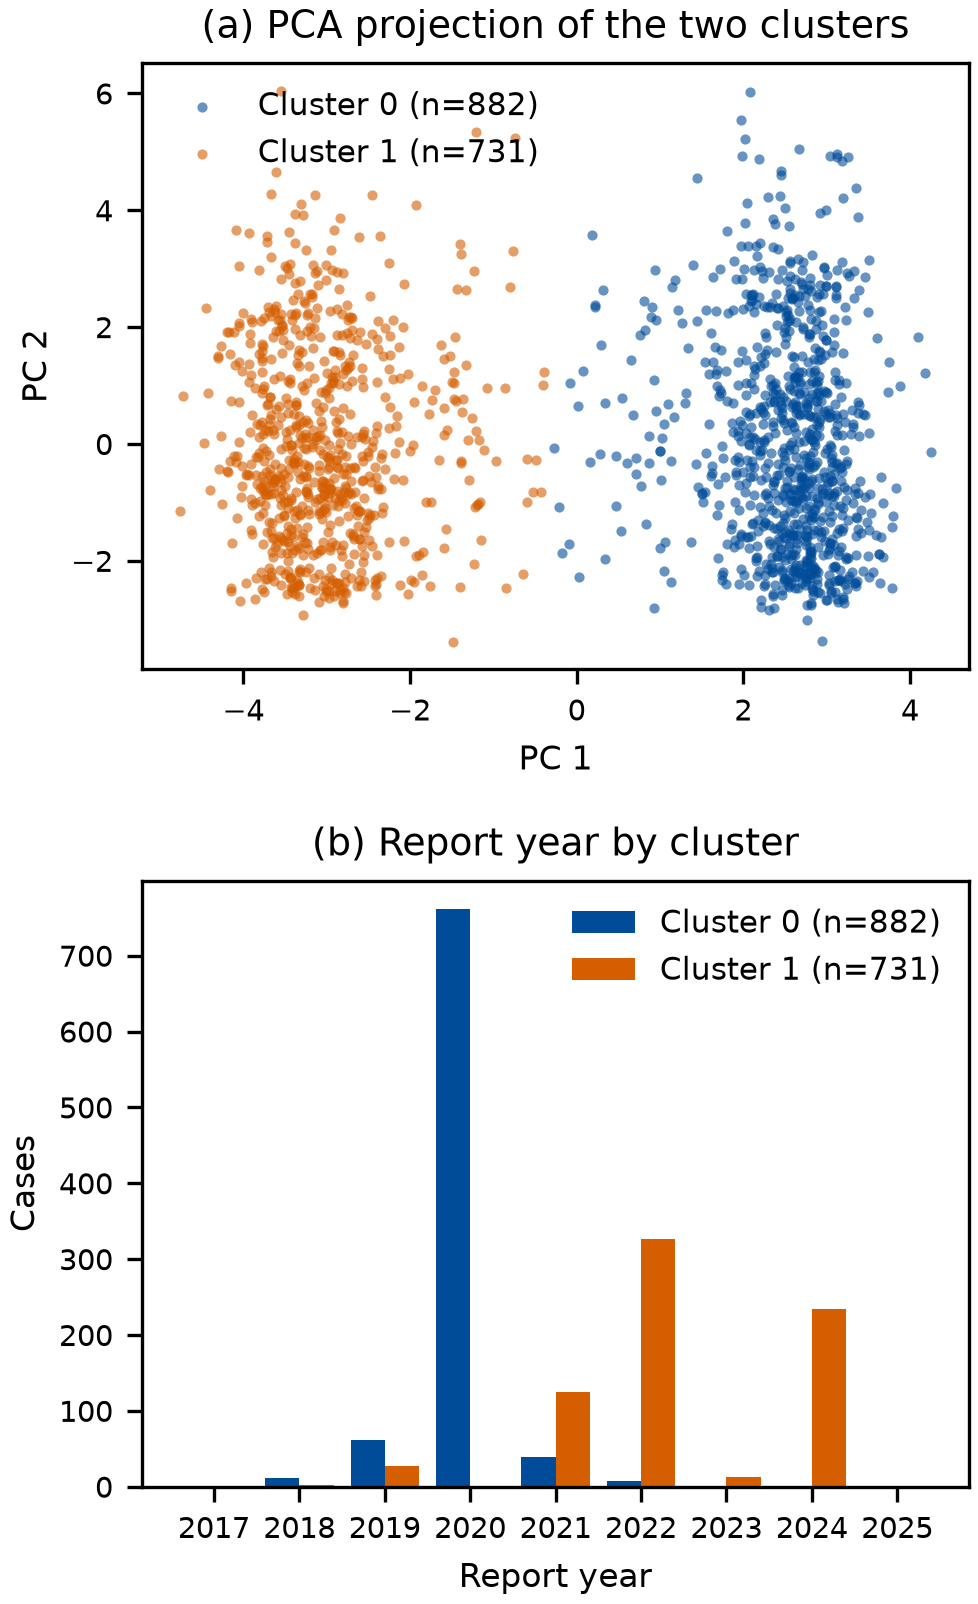
\includegraphics[width=0.80\columnwidth,keepaspectratio]{clusters_micekm.png}
\caption{MICE/KM clusters. (a) PCA projection coloured by cluster label. (b) Report-year distribution per cluster.}
\label{fig:clusters}
\end{figure}

No temporal or source field was given to the algorithms, so this split is emergent, and it shows that imputation preserved the cohort-level structure. This is the paper's central result. Principled imputation makes severely incomplete news data usable for unsupervised analysis, and the gain over dropping data holds no matter how the metrics are weighted. The source-cohort confound affects what the clusters mean, not whether imputation helps, so we claim structure recovery, not epidemiological discovery. The boundary most likely marks a change in how the data were gathered, the 2020 public collection against the later manual collection, rather than a real epidemiological divide. The cluster profiles also rest on imputed values, so they carry imputation uncertainty and describe structure rather than observed fact. Our validity indices measure only the geometric quality of the clusters, not public-health or epidemiological validity. Finer contrasts such as the workplace profile differ between pipelines, so we do not over-read them, and a cohort-aligned demographic contrast would need homogeneously sourced data before it could guide prevention. With a single run per pipeline, we also do not claim the leaders are statistically distinguishable.


\section{Conclusion}
\label{sec:conclusion}\label{sec:limitation}
Our pipeline turns severely incomplete newspaper-reported suicide data into a usable basis for unsupervised analysis, the obstacle that keeps such data out of standard machine-learning workflows. We assembled a dataset for a regime that prior work had not treated as a modelling problem, then benchmarked three imputers against no-imputation baselines under a balance-aware score tested across $100{,}000$ weightings. Earlier work clustered complete records or benchmarked imputation on artificially removed values, so none faced organically incomplete news data. Imputation improves cluster validity in over $99.9\%$ of weightings, and the strong pipelines recover the same cohort-aligned structure. Careful imputation is therefore a feasible foundation for suicide surveillance under SDG-3.

The work has clear limits. The missing values are organically absent, so there is no ground truth for imputation accuracy, and we claim usable structure rather than accurate reconstruction of individual cells. The imputers assume the missingness is ignorable. Under a missing-not-at-random mechanism, which is likely here, they can distort the least-reported fields such as occupation and circumstances, so we read those imputed fields as support for structure, not as reliable values. The recovered split also tracks the source cohort, so the cluster contrasts are confounded with collection source and should not be read as epidemiology. Newspaper reports are a selection-biased sample too. Which deaths get reported depends on location, gender, age, and method, and imputation cannot correct that bias. The corpus has no population denominator, so it cannot estimate suicide incidence or prevalence. Each pipeline was run once without resampling, and the corpus covers only cases that reached the news.

Future work broadens the method grid to more imputers and clustering families. It runs a mask-and-recover test that hides observed values and measures how well each imputer restores them, and it compares imputed and observed distributions directly. It adds bootstrap resampling for confidence intervals on the cluster structure, and it tests sensitivity to the category-consolidation mapping. Applying the pipeline to other low-resource, news-derived datasets would show whether these findings generalise beyond Bangladesh.


\section*{Ethics and Data Availability}
This study uses only information already published in the public press, for aggregate, exploratory public-health analysis, in keeping with responsible-reporting guidance on suicide. We report only aggregate cluster structure. Personal names were removed during cleaning, so the modelling and the released dataset carry no direct identifiers, and we do not describe methods of suicide in any way that could sensationalise them. The de-identified dataset, the category-mapping dictionaries, and all code are available at \url{https://github.com/akashmony01/imputation-clustering-comparison}.

\balance
\bibliographystyle{IEEEtran}
\bibliography{ref}

\end{document}
